%%%%%%%%%%%%%%%%%%%%%%%%%%%%%%%%%%%%%%%%%%%%%%%%%%%%%%%%%%%%%%%%%%%%%%%%%%%%%%%%
% TUM-Vorlage: Praesentation
%%%%%%%%%%%%%%%%%%%%%%%%%%%%%%%%%%%%%%%%%%%%%%%%%%%%%%%%%%%%%%%%%%%%%%%%%%%%%%%%
\input{./Ressourcen/Praesentation/Praeambel16zu9.tex} % Seitenverhaeltnis 16:9
\input{./_Einstellungen.tex}

\renewcommand{\PersonVorname}{Group W3}
\renewcommand{\PersonNachname}{Gallob}

\usepackage{csquotes}
\usepackage[backend=biber]{biblatex} % Stil nach Wahl
\usepackage{hyperref}
\addbibresource{resources.bib} % Hier MIT Dateiendung .bib

\input{./Ressourcen/Praesentation/Anfang.tex}

\renewcommand{\LehrstuhlName}{Chair of Connected Mobility}
\renewcommand{\FakultaetName}{School of Computation, Information and Technology}

\title{User Control in Tourism Recommender Systems}
\subtitle{Final Project Milestone \& Implementation}
\author{Group W3}
\institute[]{\UniversitaetName \\ \FakultaetName \\ \LehrstuhlName}
\date[\today]{Munich, \today}
\subject{Lab Course: Projects in Recommender Systems}
\PraesentationMasterStandard
\PraesentationTitelseite

% Slide 1: Project Overview & Motivation
\begin{frame}
    \frametitle{Last Milestone's Issues}
    \begin{itemize}
        \item Issues with calculations (occasional crashes)
        \item overloaded transparency board
        \item transparency correct only for MAUT (1st Algorithm)
    \end{itemize}
    \begin{center}
        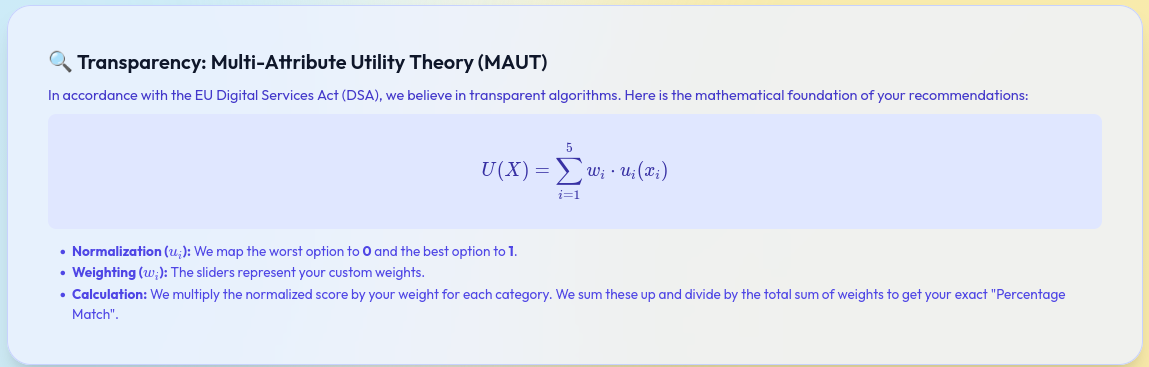
\includegraphics[width=0.7\textwidth, keepaspectratio] {screens/AlgoInfo.png}
        \begin{figure}
            \tiny\caption{Overloaded Transparency Panel}
        \end{figure}
    \end{center}
\end{frame}

\begin{frame}
    \frametitle{What The Finished App Looks Like}
    \vspace{0.8em}
    \begin{columns}
        \begin{column}{0.48\textwidth}
            \textbf{Interface Features:}
            \begin{itemize}
                \item Correct Transparency panels for MAUT and Constraint-Filtering.
                \item New Button shows Mathematical Info only on user-intent.
                \item Transparency panels uses simple language to explain the underlying logic.
            \end{itemize}
        \end{column}
        \begin{column}{0.48\textwidth}
            \begin{center}
                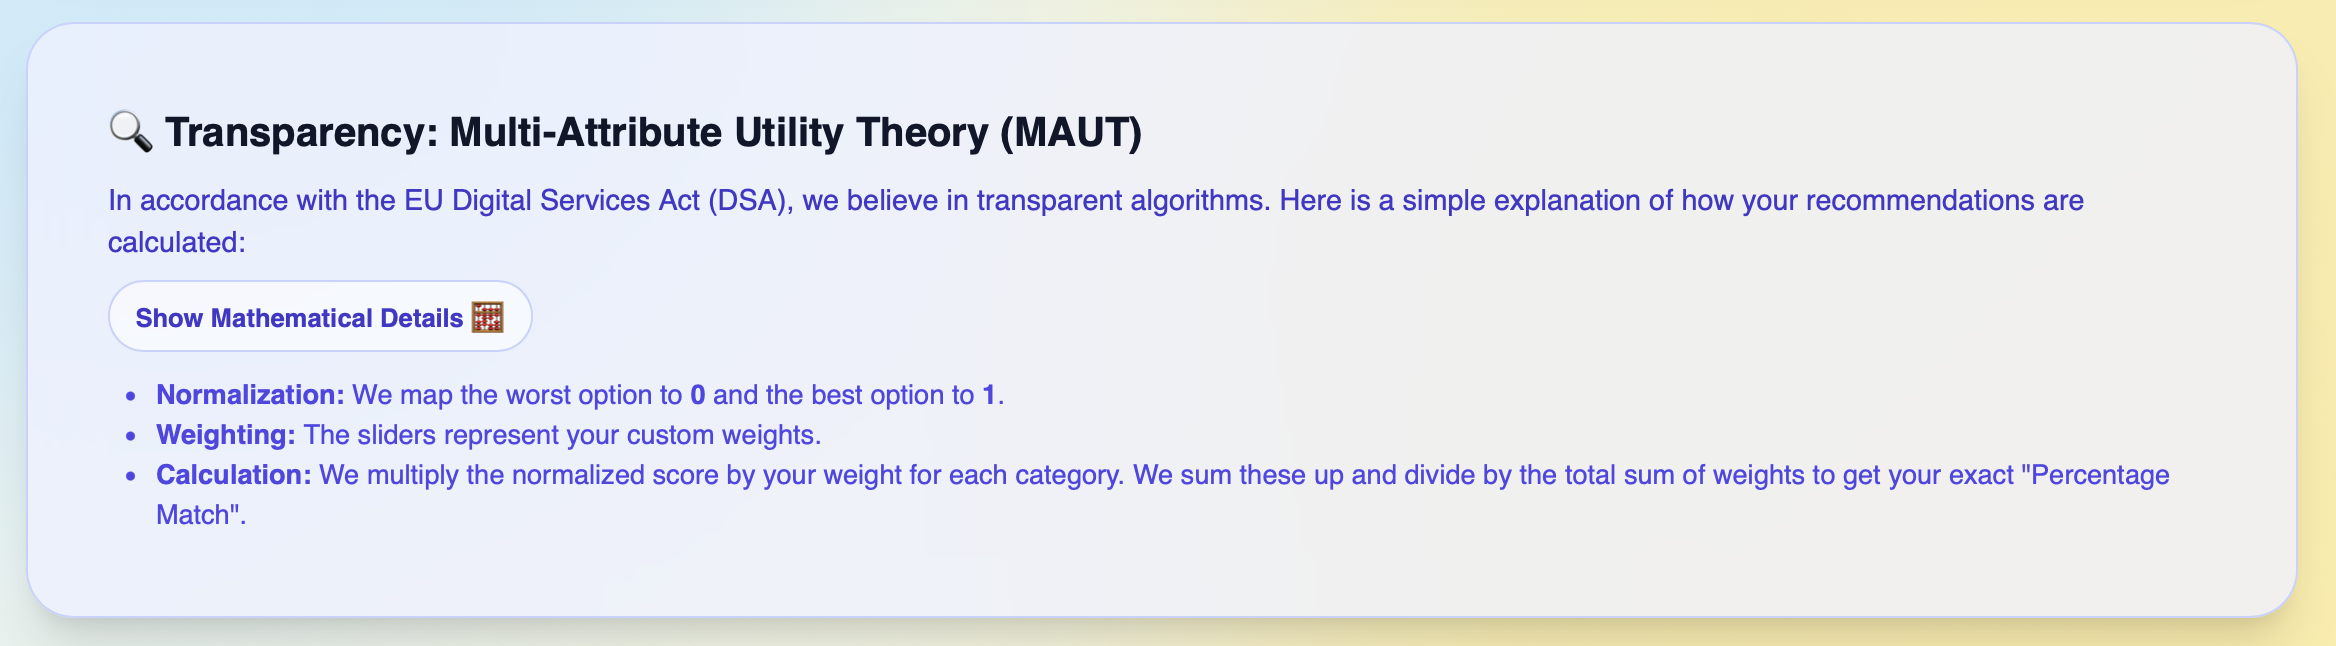
\includegraphics[width=\textwidth,keepaspectratio]{screens/newmaut.png}
                \begin{figure}
                    \tiny\caption{Transparency Board MAUT}
                \end{figure}
                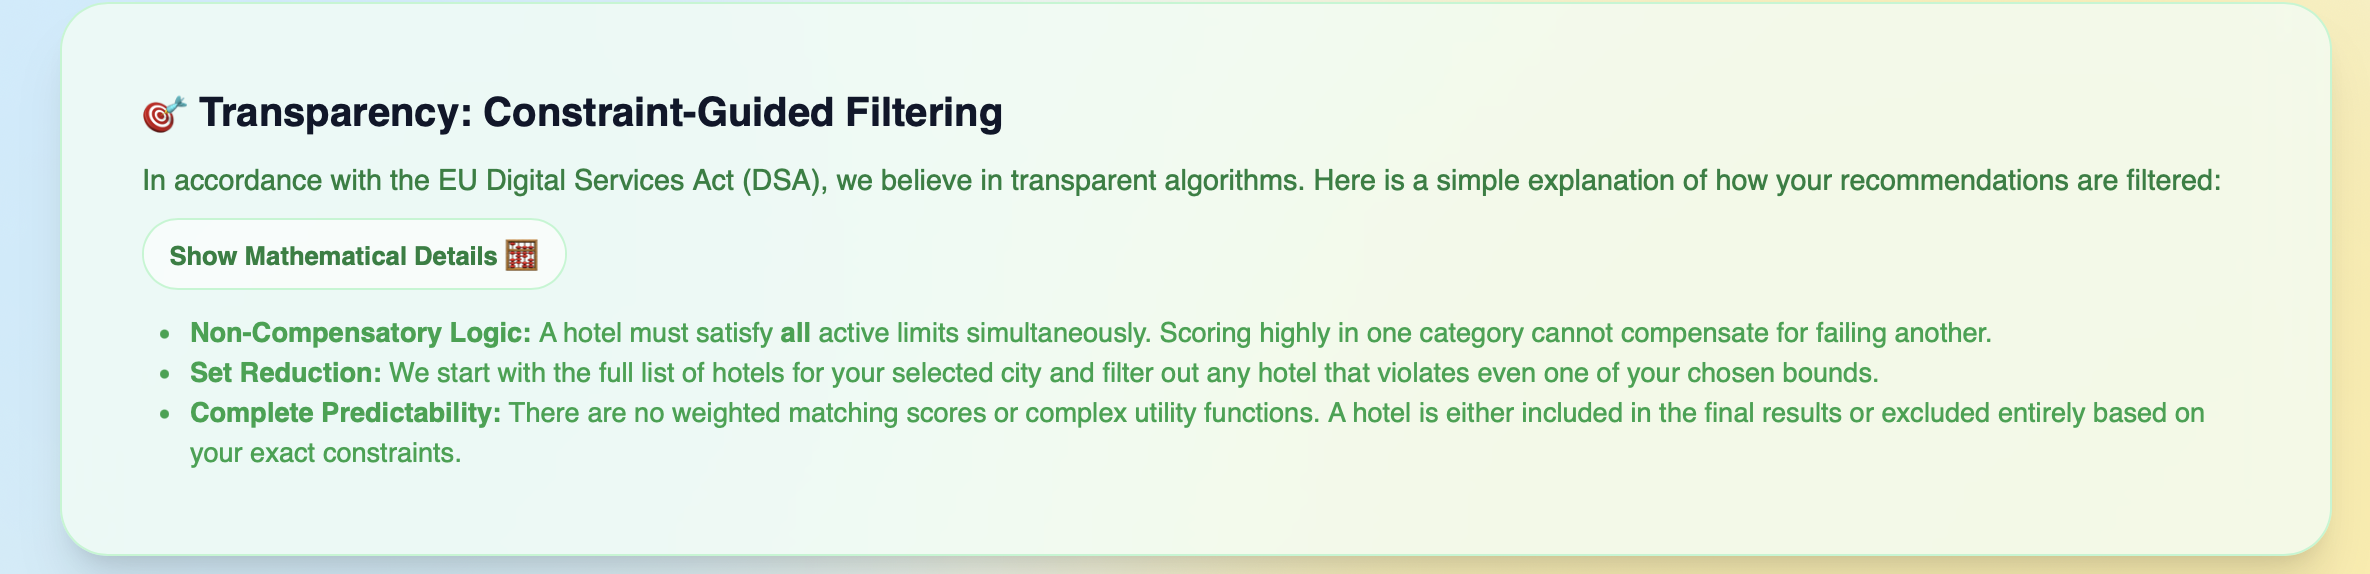
\includegraphics [width=\textwidth, keepaspectratio] {screens/Constraint.png}
                \begin{figure}
                    \tiny\caption{Transparency Board Constraint Filtering}
                \end{figure}
            \end{center}
        \end{column}
    \end{columns}
\end{frame}

\begin{frame}
    \frametitle{Explanations in simple language}
    \vspace{1em}
            \begin{block}{Algorithm A: Weighted MAUT}
                \begin{itemize}
                    \item \textbf{Normalization:} We map the worst option to 0 and the best option to 1.
                    \item \textbf{Weighting:} The sliders represent your custom weights.
                    \item \textbf{Calculation:} We multiply the normalized score by your weight for each category. We sum these up and divide by the total sum of weights to get your exact "Percentage Match".
                \end{itemize}
            \end{block}
            \begin{block}{Algorithm B: Constraint Filtering}
                \begin{itemize}
                    \item \textbf{Non-Compensatory Logic:} A hotel must satisfy all active limits simultaneously. Scoring highly in one category cannot compensate for failing another.
                    \item \textbf{Set Reduction:} We start with the full list of hotels for your selected city and filter out any hotel that violates even one of your chosen bounds.
                    \item \textbf{Complete Predictability:} There are no weighted matching scores or complex utility functions. A hotel is either included in the final results or excluded entirely based on your exact constraints.
                \end{itemize}
            \end{block}
\end{frame}

% Slide 4: User Interface & DSA Compliance (Moved up, simplified)
\PraesentationMasterWeissBlau
\begin{frame}
    \begin{center}
        \huge Demonstration
    \end{center}
\end{frame}

\PraesentationMasterStandard

% Slide 5: Implemented Algorithms

% Slide 9: Current Progress & Next Steps
\begin{frame}
    \frametitle{What's Done \& What's Next}
    \begin{itemize}
        \item \textbf{What has been achieved so far:}
            \begin{itemize}
                \item Built a UI showing real-time updates.
                \item Implemented transparency abilities to comply with DSA (collapsible breakdown panels, math display).
                \item Implemented both MAUT and hard constraint filtering modes.
                \item Fixed all issues (hopefully)
            \end{itemize}
        \item \textbf{Next step \& Possble Extensions:}
            \begin{itemize}
                \item \textbf{Finish project documentation}.
                \item \textbf{Hybrid mode:} 3rd mode, i.e. Combine both modes (filter out expensive hotels, then rank the rest using MAUT)?
                \item \textbf{Expand mock database:} Add more hotels to the mock database (i.e. 20 each) ?
            \end{itemize}
    \end{itemize}
\end{frame}

% Final Slide
\PraesentationMasterWeissBlau
\begin{frame}
    \begin{center}
        \huge Thank you for your attention! \\
        \vspace{1em}
        \large Questions?
    \end{center}
\end{frame}

\PraesentationMasterStandard
\begin{frame}[allowframebreaks]
    \frametitle{References}
    \printbibliography
\end{frame}

\end{document}
